\documentclass[tikz, border = 10pt]{standalone}

%%%<
\usepackage{verbatim}
\usetikzlibrary{calc, intersections, through}
%%%>

\begin{comment}
:Title: Ptolemy's theorem on quadrilaterals circumscribed by a circle
:Author: Moti Ben-Ari
:Tags: Geometry;Intersections;Straightedge and compass
:Slug: Ptolemy's theorem

Here are three theorems from Euclidean geometry:

  Theorem: The opposite angles of an isosceles trapezoid
    are supplementary.
  
  Theorem: A quadrilateral whose opposite angles are supplementary
    can be circumscribed by a circle.
  
  Theorem (Ptolemy): Let Q a quadrilateral circumscribed by a circle,
    let its two pairs of opposite sides be (a, b) and (c, d),
    and let its diagnonals be (e, f). Then ef = ab + cd.

The Mohr-Mascheroni Theorem shows that any construction
that can be done with straightedge and compass
can be done with a compass only!

One proof of this theorem uses Ptolemy's theorem.
The construction here is based upon the the proof presented in:
  "Surprising constructions with straightedge and compass",
  https://www.weizmann.ac.il/sci-tea/benari/mathematics,
which is based on presentations by Heinrich Doerrie and
Michael Woltermann.

TikZ features: name path, intersection, circle through,
  distance modifier, let...in, \pgfmathparse.
\end{comment}

\begin{document}
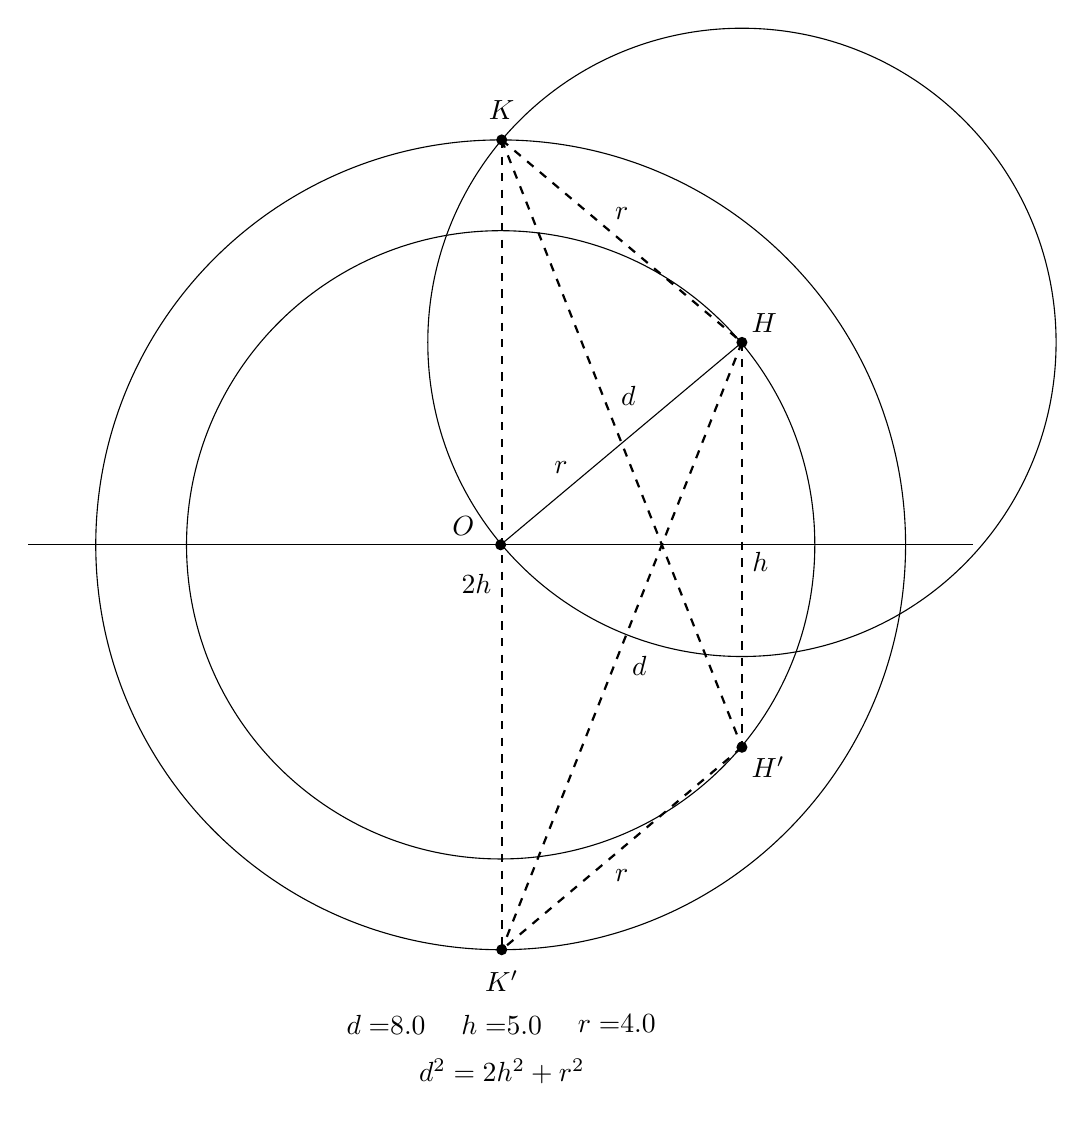
\begin{tikzpicture}

  % Label point (0, 0) by (O) and draw a horizontal line through (O).
  
  \coordinate (O) at (0, 0);
  \fill (O) node[above left, xshift=-6pt]
    {$O$} circle[radius = 2pt];
  \draw (-6, 0) -- (6, 0);
  
  % Label a point by (H) and construct a circle centered
  %   at (O) through (H). 
  % The circle path is named "circle" and its radius labeled r.
  
  \draw (O) -- node[above, near start, yshift = 4pt]
    {$r$} (40 : 4) coordinate (H);
  \fill (H) node[above right]
    {$H$} circle[radius = 2pt];
  \node[draw, circle through = (H), name path=circle] at (O) {};
  
  % Reflect point (H) about the horizontal line and label the
  %   reflected point by (Hprime).
  
  % Method:
  %   Define the coordinate (perpH) as the projection of (H) on
  %     the horizontal line and label it H' on the diagram.
  %   Use a distance modifier to construct a line twice the length
  %     of HH' through (H) and (perpH).
  %   The length HH' is labeled h.
  
  \coordinate (perpH) at (H |- O);
  \draw[thick, dashed] (H) -- node[right, yshift = -6pt]
    {$h$} ($(H) ! 2 ! (perpH)$) coordinate (Hprime);
  \fill (Hprime) node[below right]
    {$H'$} circle[radius = 2pt];
  
  % Construct a circle centered at (H) whose radius is r,
  %   the same as the radius of "circle".
  % The circle path is named "circleR".
  
  % Method:
  %   (H) - (O) is the length of the radius r.
  %   let...in with veclen obtains this length.
  
  \path[draw, name path = circleR] (H)
  let
    \p1 = ($ (H) - (O) $)
  in
    circle ({veclen(\x1, \y1)});
  
  % Similarly, construct a circle centered at (O) with
  %   radius (H) - (Hprime), which has been labeled h.
  % The circle path is named "circleH".
  
  \path[draw, name path = circleH] (O)
  let
    \p1 = ($ (H) - (Hprime) $)
  in
    circle ({veclen(\x1, \y1)});
  
  % Construct point (K) as the intersection of circleR and circleH.
  
  \path [name intersections = 
          {of = circleR and circleH,
           by = {K}}];
  \fill (K) node[above, yshift = 4pt]
    {$K$} circle[radius = 2pt];
  
  % Construct (Kprime), the reflection of (K) about the horizontal line,
  %   using the method for obtaining (Hprime) from (H).
  % The length of (K) - (Kprime) is 2h since the radius of
  %   circle H is h.
  
  \coordinate (perpK) at (K |- O);
  \draw[thick, dashed] (K) --  node[left, yshift = -14pt]
    {$2h$} ($ (K) ! 2 ! (perpK) $) coordinate (Kprime);
  \fill (Kprime) node[below, yshift = -4pt]
    {$K'$} circle[radius = 2pt];
  
  % Label HK by the radius r.
  % Since (Hprime) is the reflection of (H) and 
  %   (Kprime) is the reflection of (K),
  %   it can be proved that the length H'K' is also r.
  
  \draw[thick, dashed] (K) -- node[above, yshift = 4pt]
    {$r$} (H);
  \draw[thick, dashed] (Hprime) -- node[below, yshift = -4pt]
    {$r$} (Kprime);
  
  % The result of the construction is an isoceles trapezoid KHH'K'
  %   displayed with dashed lines.
  
  % Construct the diagonals KH' and K'H.
  % Since the trapezoid is isoceles, the diagonals are of equal
  %   length labeled d.
  
  \draw[thick, dashed] (K) --
    node[above right, xshift = -4pt, yshift = 10pt]
    {$d$} (Hprime);
  \draw[thick, dashed] (H) -- node[below right]
    {$d$} (Kprime);
  
  % Check that Ptolemy's Theorem holds by computing and
  %   displaying d, h, r.
  
  % Method:
  %   let...in with veclen obtains the length of each line segment.
  %   The length is multiplied by 0.03528 to convert points to cm
  %     and rounded.
  %   \pgfmathparse and \pgfmathresult are used to display the lengths.
  %   The values are displayed at the bottom of the diagram, below K'.
  
  % d is KH'.
  
  \draw (Kprime)
    let
      \p1 = ($ (K) - (Hprime) $)
    in
    node[below left, xshift = -24pt, yshift = -20pt]
      {$d = $\pgfmathparse{
           round(
             veclen(\x1, \y1) * 0.03528
           )
         }
         \pgfmathresult
    };

  % h is HH'.
  
  \draw (Kprime)
    let
      \p1 = ($ (H) - (Hprime) $)
    in
    node[below, yshift = -20pt]
      {$h = $\pgfmathparse{
           round(
             veclen(\x1, \y1) * 0.03528
           )
         }
         \pgfmathresult
    };
  
  % r is KH.
  
  \draw (Kprime)
    let
      \p1 = ($ (K) - (H) $)
    in
    node[below right, xshift = 24pt, yshift = -20pt]
      {$r = $\pgfmathparse{
           round(
             veclen(\x1, \y1) * 0.03528
           )
         }
         \pgfmathresult
    };
  
  % Display the equation from Ptolemy's Theorem.
  % Within a reasonable error, the equation holds.
  
  \draw (Kprime) node[below, yshift = -36pt] 
    {$d^2=2h^2+r^2$};

\end{tikzpicture}

\end{document}
